\begin{apendicesenv}

\partapendices

\chapter{Algoritmos e Repositórios}
\label{ap:algoritmos}

Este apêndice reúne os detalhes de implementação que sustentam o Capítulo~\ref{cap:metodologia}: os repositórios em que o código e os dados estão publicados, a organização dos dados em camadas, o procedimento de agregação mesorregional, o cálculo das métricas de pico e de estabilidade distribucional e a função de cada script da pipeline v4.

\section{Repositórios e Dados Publicados}
\label{ap:repositorios}

\begin{itemize}
    \item \textbf{Código da pipeline e do painel:} repositório MODELO-PREVISAO~\cite{modeloprevisao2026}, com os scripts, a configuração da divisão temporal (\texttt{config/recorte.json}), os relatórios JSON de cada etapa e o código do painel.\newline \url{https://github.com/modelo-previsao-dengue/MODELO-PREVISAO}
    \item \textbf{Texto da monografia:} repositório TCC2-DOCS, com o código-fonte \LaTeX{}, as figuras e o arquivo \texttt{RASTREABILIDADE.md}, que relaciona cada número do texto ao relatório que o produziu.\newline \url{https://github.com/modelo-previsao-dengue/TCC2-DOCS}
    \item \textbf{Dados e modelos:} HuggingFace Datasets, com as camadas Bronze, Silver e Gold, os conjuntos de treino e teste, os modelos treinados e os relatórios.\newline \url{https://huggingface.co/datasets/pedrolucassantanaf/dengue-tcc2-data}
    \item \textbf{Notebooks:} Kaggle.\newline \url{https://www.kaggle.com/pedrolucassantana}
    \item \textbf{Painel interativo:} Streamlit Community Cloud.\newline \url{https://modelo-previsao-ffqc3ugltpbxxeaa4mygvw.streamlit.app}
\end{itemize}

\section{Organização dos Dados em Camadas}
\label{ap:camadas}

Os dados de ambas as fontes foram organizados segundo a arquitetura em camadas Bronze, Silver e Gold, armazenadas em formato Parquet. Cada execução gera uma versão nomeada (por exemplo, \texttt{sinan\_tcc2\_v2}), o que permite reproduzir qualquer resultado a partir da versão correspondente.

\begin{itemize}
    \item \textbf{Bronze:} os arquivos originais, sem transformação de conteúdo. No SINAN, os microdados anuais de dengue do OpenDataSUS, inventariados com origem, tamanho e soma de verificação (\textit{checksum}); no INMET, os arquivos horários das estações automáticas.
    \item \textbf{Silver:} os dados limpos e padronizados. No SINAN, datas, tipos e códigos territoriais normalizados, duplicidades exatas removidas, registros sem semana epidemiológica ou município válidos descartados com registro do descarte, e uma linha por município e semana de notificação; no INMET, colunas mapeadas para nomes padronizados, o valor sentinela $-9999$ convertido em ausente e agregação por estação e semana epidemiológica.
    \item \textbf{Gold:} os dados prontos para a modelagem. No SINAN, a contagem de notificações e os atributos clínicos e demográficos por município de residência e semana de notificação, em grade densa, com as semanas sem notificação preenchidas com zero. No INMET, a camada Silver já é a entrada da agregação mesorregional.
\end{itemize}

\section{Agregação Mesorregional}
\label{ap:agregacao}

A série de modelagem foi construída pelos passos a seguir.

\begin{enumerate}
    \item Cada estação do INMET é associada ao município mais próximo, pela distância haversine entre as coordenadas da estação e as do município, e, por meio dele, à sua mesorregião, segundo a hierarquia do IBGE.
    \item Cada município do SINAN é associado à sua mesorregião pela mesma hierarquia.
    \item Para cada mesorregião e semana epidemiológica, as contagens de notificações dos municípios são somadas, e as proporções e os índices clínicos são combinados por média ponderada pelo número de notificações de cada município.
    \item Para cada mesorregião e semana epidemiológica, cada variável climática é a média aritmética simples das estações da mesorregião com dado naquela semana. Se nenhuma estação tem dado, a variável fica ausente.
    \item As duas séries são unidas pela chave (mesorregião, ano epidemiológico, semana epidemiológica), mantendo todas as semanas da série epidemiológica. Um indicador binário registra se a semana tem dado climático; ele é usado apenas como metadado, e não como atributo do modelo.
    \item Como verificação, a execução é interrompida se houver chaves duplicadas ou se o número de mesorregiões for diferente de 137, e a soma das notificações das mesorregiões em cada ano é comparada com o total da camada Gold.
\end{enumerate}

\section{Métricas de Pico e de Estabilidade Distribucional}
\label{ap:metricas}

\paragraph{Erro na semana do pico.} Para cada mesorregião $m$ e temporada $s$ (ano epidemiológico) com ao menos uma semana no nível de risco mais alto, sejam $y_{m,s}(w)$ e $\hat{y}_{m,s}(w)$ as notificações observadas e previstas na semana $w$. O erro na semana do pico é
\begin{equation}
e_{m,s} = \mathop{\mathrm{arg\,max}}_{w} \hat{y}_{m,s}(w) - \mathop{\mathrm{arg\,max}}_{w} y_{m,s}(w),
\end{equation}
em semanas. Valores positivos indicam pico previsto depois do observado. São reportados a proporção de temporadas com $|e_{m,s}| \leq 2$, a mediana de $|e_{m,s}|$ e a média de $e_{m,s}$.

\paragraph{\textit{Population Stability Index} (PSI).} Para cada atributo, a distribuição do conjunto de teste é tomada como referência e dividida em $k=10$ faixas pelos seus decis (faixas com limites repetidos são unidas; se restarem menos de duas faixas, o PSI é zero). Em seguida, conta-se quantos valores de cada ano de treino caem em cada faixa. Com $n_i$ e $N$ o número de valores na faixa~$i$ e o total, as proporções são suavizadas por
\begin{equation}
p_i = \frac{n_i + 1}{N + k},
\end{equation}
o que evita divisões por zero em faixas vazias. Com $r_i$ as proporções da referência e $a_i$ as do ano comparado,
\begin{equation}
\mathrm{PSI} = \sum_{i=1}^{k} (a_i - r_i) \ln\frac{a_i}{r_i}.
\end{equation}
O cálculo foi feito para os 20 atributos mais importantes segundo os valores SHAP. Valores acima de 0,25 indicam mudança relevante de distribuição.

\section{Scripts da Pipeline v4}
\label{ap:scripts}

A Tabela~\ref{tab:scripts} lista os scripts da pipeline v4, na pasta \texttt{scripts/} do repositório MODELO-PREVISAO. Os scripts 40 a 55 formam a pipeline principal, executada em sequência; os scripts 56 a 63 são análises complementares sobre os dados e os modelos gerados por ela.

\begin{table}[htbp]
\centering
\caption{Scripts da pipeline v4 e respectivas funções}
\label{tab:scripts}
\footnotesize
\begin{tabular}{|c|p{0.80\textwidth}|}
\hline
\textbf{Script} & \textbf{Função} \\ \hline
40 & Agrega o SINAN (camada Gold) por mesorregião e semana epidemiológica, de 2000 a 2026. \\ \hline
41 & Agrega o INMET (camada Silver) por mesorregião e semana epidemiológica e registra os anos sem dados. \\ \hline
42 & Integra as séries do SINAN e do INMET e adiciona o indicador de presença de dado climático. \\ \hline
43 & Gera as defasagens de 1 a 8 semanas e as médias móveis. \\ \hline
44 & Gera as anomalias climáticas em relação à climatologia do período de treino. \\ \hline
45 & Separa treino, validação e teste para as três janelas temporais (curta, longa e longa ponderada). \\ \hline
46 & Treina os nove modelos de regressão (três janelas $\times$ três conjuntos de atributos) e calcula os intervalos de confiança por \textit{bootstrap}. \\ \hline
47 & Executa a validação \textit{walk-forward}. \\ \hline
48 & Calcula a importância dos atributos (ganho e valores SHAP). \\ \hline
49 & Otimiza os hiperparâmetros com Optuna. \\ \hline
50 & Calcula a estabilidade distribucional dos atributos (PSI e teste de Kolmogorov--Smirnov). \\ \hline
51 & Gera a curva de aprendizado em função do tamanho da janela de treino. \\ \hline
52 & Compila os resultados da pipeline em um relatório único. \\ \hline
53 & Gera as tabelas e figuras usadas no texto. \\ \hline
54 & Treina os classificadores do nível de risco. \\ \hline
55 & Gera a página estática do painel com as previsões e os alertas. \\ \hline
56 & Análises complementares: baselines ingênuos, métricas de momento, alertas, cenários de atraso na notificação e recorte do Distrito Federal. \\ \hline
57 & Avalia os modelos salvos, sem retreino: baselines, métricas por ano, métricas de momento, recorte do Distrito Federal e série nacional. \\ \hline
58 & Avalia o vazamento temporal dos atributos clínicos da semana~$t$ e treina o modelo realista. \\ \hline
59 & Calcula os baselines avançados (climatologia e Ridge) e os controles de região e semana. \\ \hline
60 & Calcula o MASE por mesorregião e os testes de Diebold--Mariano com \textit{bootstrap} em blocos. \\ \hline
61 & Compara a classificação do nível de risco com os baselines e mede a antecedência da sinalização de subida. \\ \hline
62 & Testa formalmente a contribuição do clima (Diebold--Mariano e \textit{bootstrap} em blocos). \\ \hline
63 & Refaz os cenários de atraso na notificação com o conjunto de atributos realista. \\ \hline
\end{tabular}
\fonte{Repositório MODELO-PREVISAO~\cite{modeloprevisao2026}.}
\end{table}

\chapter{Comparação com a Pipeline Anterior às Correções (v3)}
\label{ap:comparacao_v3}

Este apêndice apresenta os resultados obtidos com a pipeline anterior às correções de dados descritas na Seção~\ref{sec:correcoes}. Na versão anterior (v3), a janela de treino cobria 2019 a 2022 (4~anos), e os modelos diferiam apenas no \textbf{conjunto de atributos}: só SINAN, SINAN + INMET bruto e SINAN + INMET enriquecido. Neste apêndice, os modelos da v3 são identificados por esse conjunto; as letras A, B e C são usadas apenas no corpo do trabalho, para as variantes de janela temporal da v4. Os números abaixo servem como referência para dimensionar o efeito das correções.

\section{Efeito das Correções sobre os Resultados de Regressão}

A Tabela~\ref{tab:antes_depois} compara a mesma pipeline executada antes e depois das correções, com o mesmo conjunto de teste. As correções melhoraram o desempenho de todas as variantes, e duas conclusões se inverteram. Primeiro, o clima passou a ajudar de forma significativa nos cenários de atraso na notificação, nos quais antes a diferença era negativa e não significativa. Segundo, a variável climática mais associada aos casos deixou de ser a ``umidade'', cujo limiar de 15,7\% era, na verdade, uma temperatura de ponto de orvalho em graus Celsius, e passou a ser a temperatura mínima, com limiar fisicamente plausível.

\begin{table}[htb]
\centering
\caption{Resultados da pipeline mesorregional antes e depois das correções de dados}
\label{tab:antes_depois}
\small
\begin{tabular}{|p{0.44\textwidth}|c|c|}
\hline
\textbf{Indicador} & \textbf{Antes} & \textbf{Depois} \\ \hline
$R^2_{\log}$ do modelo só SINAN & 0,843 & 0,859 \\ \hline
$R^2_{\log}$ do modelo SINAN + INMET enriquecido & 0,853 & 0,870 \\ \hline
Ganho do clima com atraso de 4 semanas ($\Delta R^2_{\log}$) & $-$0,0006 ($p=0{,}60$) & +0,0047 ($p<0{,}001$) \\ \hline
Ganho do clima com atraso de 8 semanas ($\Delta R^2_{\log}$) & $-$0,0013 ($p=0{,}22$) & +0,0035 ($p<0{,}001$) \\ \hline
\textit{Walk-forward}: janelas em que C supera A & 3 de 5 & 4 de 4 \\ \hline
Melhor variável climática no SHAP (posição) & pressão (12.ª) & temp. mínima (20.ª) \\ \hline
Limiar climático de destaque & ``umidade'' 15,7 & temp. mínima 13,8~$^\circ$C \\ \hline
\end{tabular}
\fonte{Dados do SINAN (DATASUS) e do INMET, 2000--2026.}
\nota{Antes: relatórios do PR \#1 do repositório MODELO-PREVISAO~\cite{modeloprevisao2026}; depois: pipeline reprocessada.}
\end{table}

\section{Classificação do Nível de Risco (v3)}

Na pipeline v3, com janela curta de treino (2019--2022), os classificadores XGBoost, um para cada conjunto de atributos, foram avaliados com os mesmos baselines.

Na classificação em quatro níveis de risco (Tabela~\ref{tab:risco_v3}), o XGBoost dedicado alcançou F1 macro de 0,49 e AUC de 0,77 com clima, contra 0,47 e 0,75 sem clima. Todos os classificadores, no entanto, ficaram abaixo da simples aplicação dos limiares de risco à persistência, que obteve F1 macro de 0,62 e foi superior em todas as classes. As classes intermediárias (moderado e alto) foram as mais difíceis para todos os métodos.

\begin{table}[htb]
\centering
\caption{Classificação do nível de risco no conjunto de teste --- pipeline v3 (F1)}
\label{tab:risco_v3}
\small
\begin{tabular}{|l|c|c|c|c|c|}
\hline
\textbf{Modelo} & \textbf{Macro} & \textbf{Baixo} & \textbf{Moderado} & \textbf{Alto} & \textbf{Muito alto} \\ \hline
Persistência & \textbf{0,622} & \textbf{0,837} & \textbf{0,481} & \textbf{0,416} & \textbf{0,755} \\ \hline
Média móvel (4 semanas) & 0,578 & 0,810 & 0,431 & 0,372 & 0,700 \\ \hline
XGBoost, só SINAN & 0,470 & 0,724 & 0,286 & 0,263 & 0,609 \\ \hline
XGBoost, + INMET bruto & 0,491 & 0,740 & 0,323 & 0,268 & 0,632 \\ \hline
XGBoost, + INMET enriquecido & 0,491 & 0,736 & 0,299 & 0,284 & 0,643 \\ \hline
\end{tabular}
\fonte{Dados do SINAN (DATASUS) e do INMET, 2000--2026.}
\end{table}

O experimento complementar chegou ao mesmo resultado com uma definição de surto diferente, binária e baseada no canal endêmico: o classificador dedicado obteve F1 de 0,72 a 0,74 para a classe surto, abaixo da persistência do rótulo (0,85). Aplicar o limiar do canal endêmico à previsão contínua da regressão, em vez de treinar um classificador, alcançou 0,83, próximo à persistência. Os dois resultados indicam que, para gerar alertas, é preferível derivá-los da previsão numérica, e não treinar um classificador separado.

\section{Interpretação do Modelo --- SHAP (v3)}

A análise SHAP da variante com clima enriquecido na v3 (Figura~\ref{fig:shap_v3}) mostra que a previsão é dominada pela própria série epidemiológica: as notificações da semana anterior respondem sozinhas por uma contribuição média (1,15) mais de quatro vezes maior que a segunda variável, a codificação cíclica da semana ($\cos$: 0,26). A diferença de notificações entre semanas ($0{,}17$), a contagem de confirmados/prováveis ($0{,}12$) e a média móvel de 2 a 4~semanas ($0{,}10$) completam as cinco mais importantes. Nenhuma variável climática aparece entre as dez mais importantes; a primeira é a temperatura mínima da semana, na 20.ª posição.

\begin{figure}[htb]
    \centering
    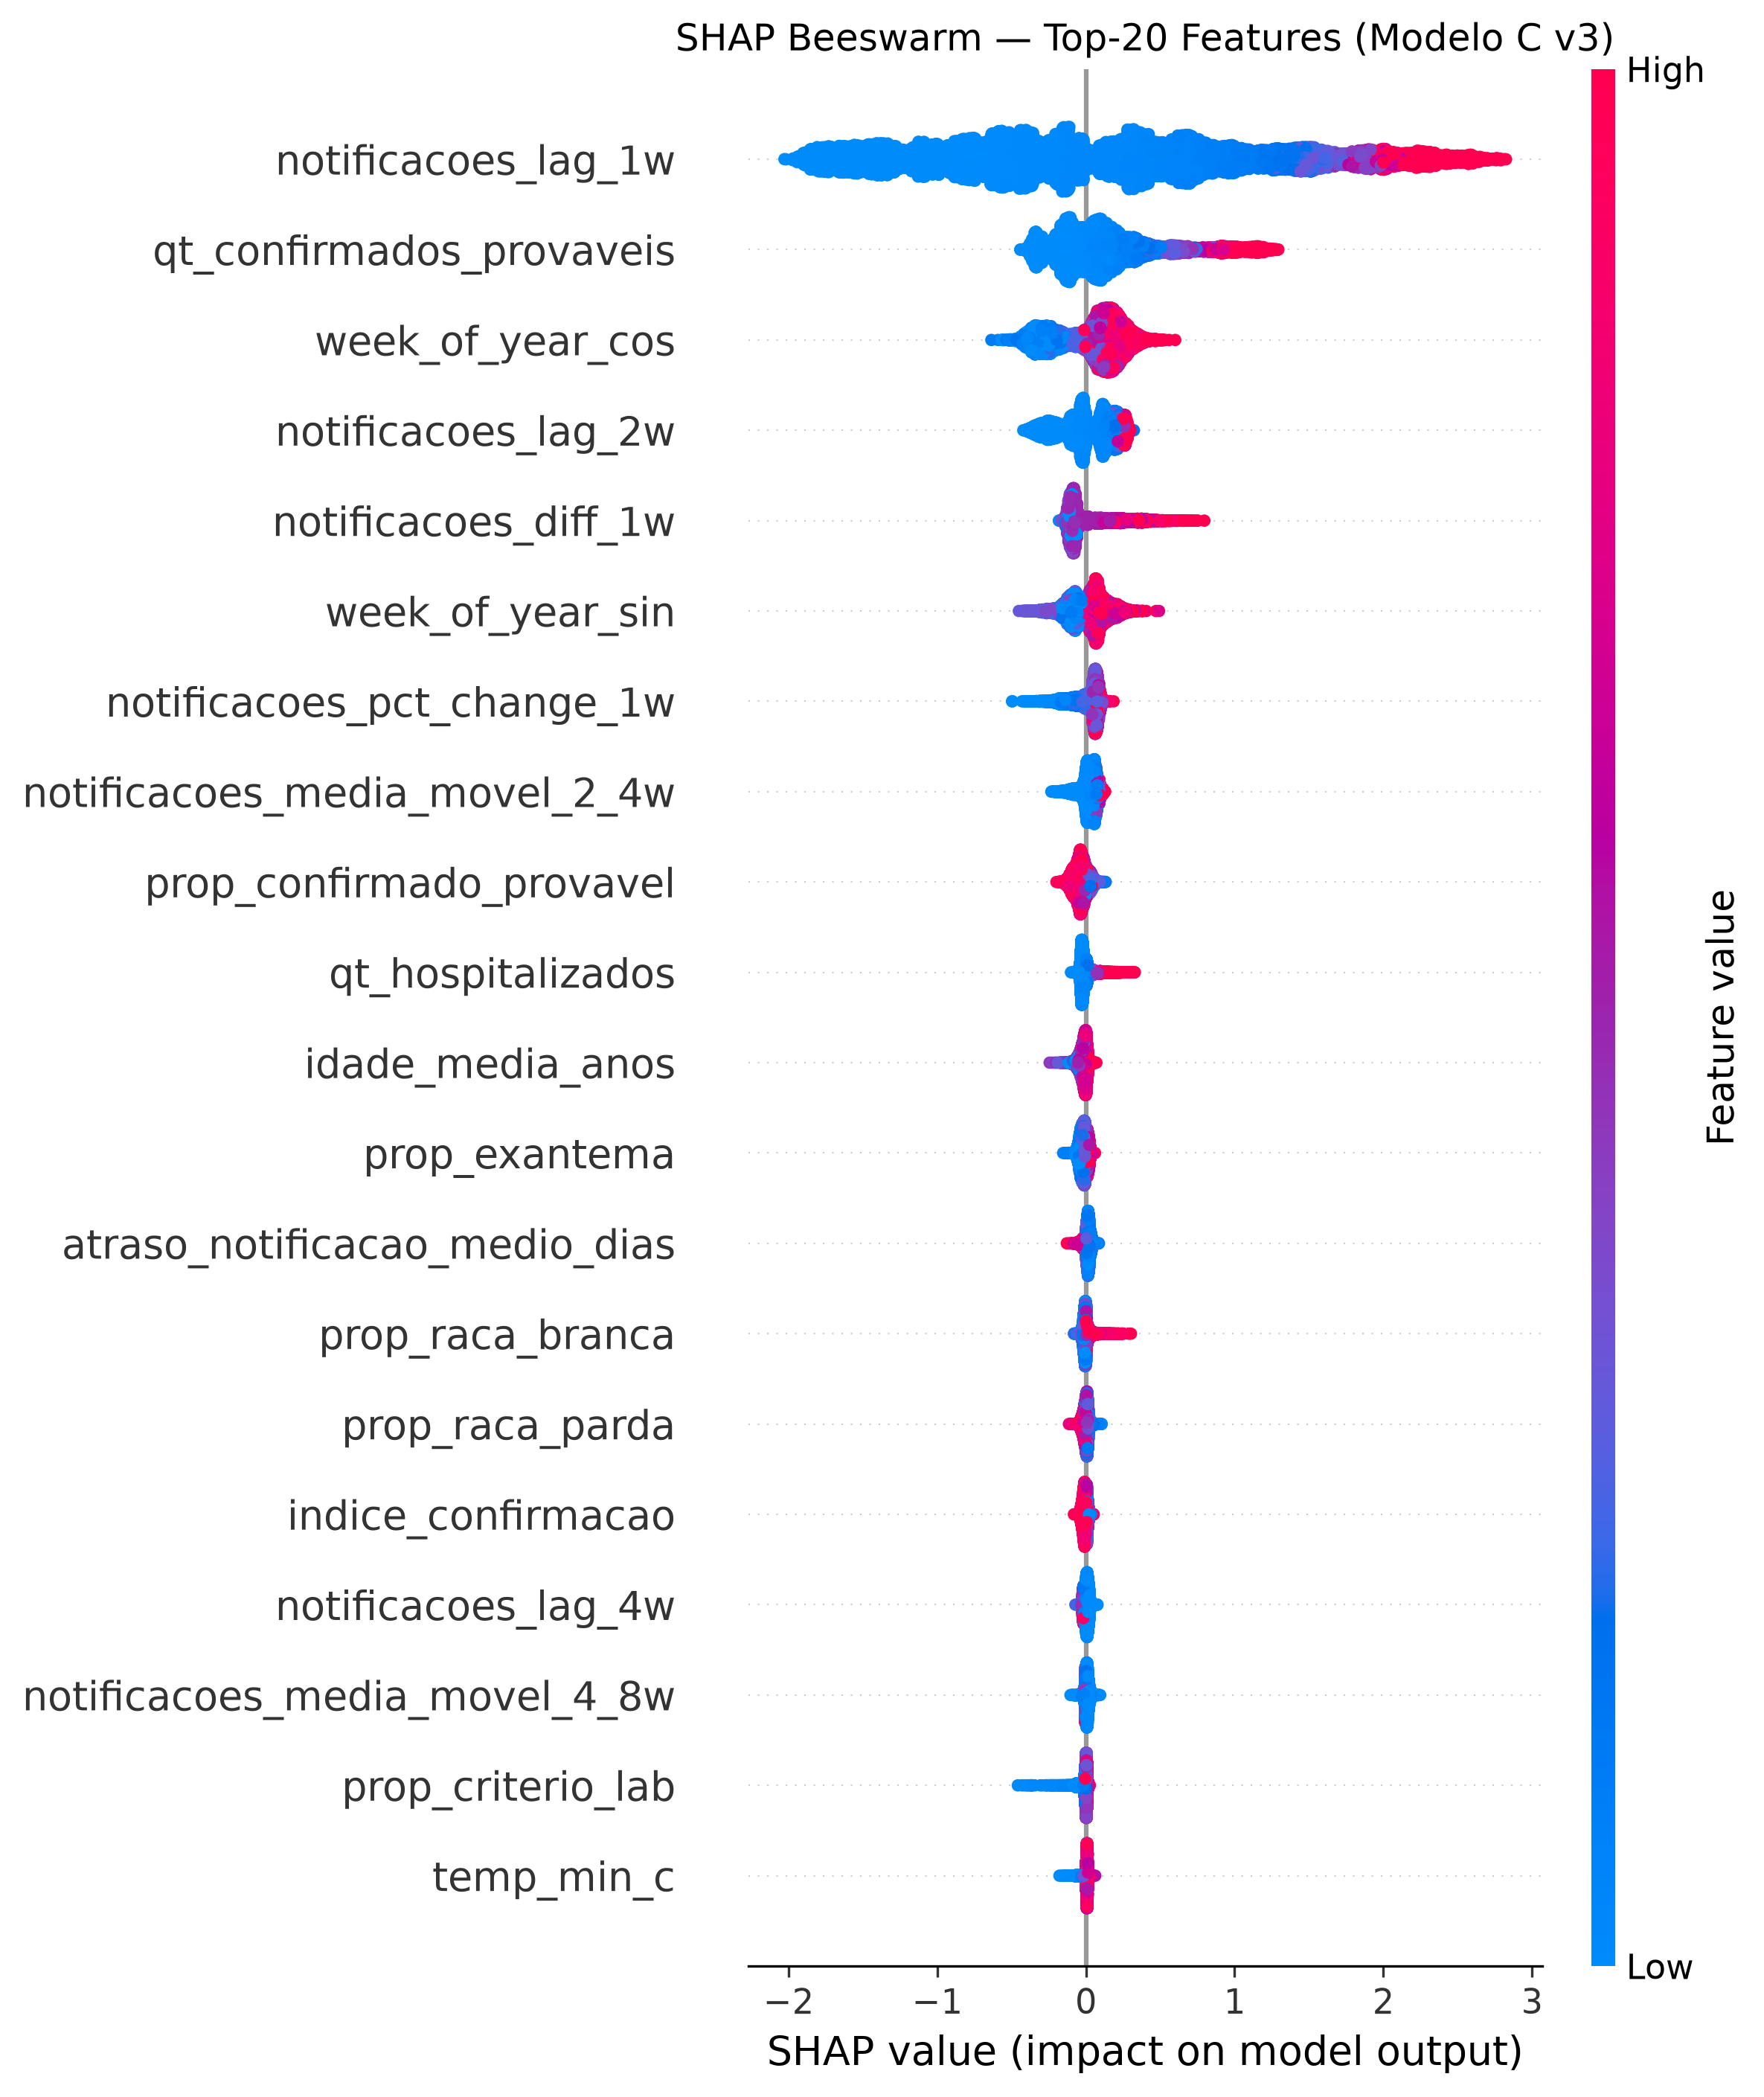
\includegraphics[width=0.7\textwidth]{figuras/resultados/fig_v3_shap_beeswarm.png}
    \caption{Valores SHAP das 20 variáveis mais importantes do modelo com INMET enriquecido --- pipeline v3}
    \label{fig:shap_v3}
    \fonte{Dados do SINAN (DATASUS) e do INMET, 2000--2026.}
    \nota{No título da figura, ``Modelo C'' é o rótulo da v3 para o modelo com INMET enriquecido.}
\end{figure}

Os limiares estimados para as variáveis climáticas (Tabela~\ref{tab:limiares_v3}) são coerentes com a biologia do vetor. A contribuição da temperatura passa a ser positiva acima de 13,8~$^\circ$C de mínima e de 21,0~$^\circ$C de média semanal, valores próximos do limite inferior de transmissão descrito na literatura. A precipitação média na janela de 2 a 4 semanas e o número de dias de chuva nessa janela aumentam a previsão, o que corresponde ao intervalo de desenvolvimento do vetor. A pressão atmosférica tem efeito negativo, provavelmente como indicador indireto de altitude e de massas de ar mais secas e frias.

\begin{table}[htb]
\centering
\caption{Limiares climáticos estimados pela análise SHAP (modelo com INMET enriquecido, v3) e efeito sobre a previsão acima do limiar}
\label{tab:limiares_v3}
\small
\begin{tabular}{|p{0.47\textwidth}|c|r|c|}
\hline
\textbf{Variável} & \textbf{Posição} & \textbf{Limiar} & \textbf{Efeito} \\ \hline
Temperatura mínima (semana $t$) & 20 & 13,8~$^\circ$C & aumenta \\ \hline
Temperatura média (semana $t$) & 21 & 21,0~$^\circ$C & aumenta \\ \hline
Precipitação média, média de 2 a 4 semanas & 22 & 0,11~mm/h & aumenta \\ \hline
Radiação média, média de 4 a 8 semanas & 23 & 1.317~kJ/m$^2$ & aumenta \\ \hline
Pressão média, 8 semanas antes & 25 & 992~hPa & reduz \\ \hline
Pressão média, média de 4 a 8 semanas & 27 & 981~hPa & reduz \\ \hline
Dias de chuva, média de 2 a 4 semanas & 28 & 2,1 dias & aumenta \\ \hline
Precipitação acumulada, média de 2 a 4 semanas & 29 & 16,1~mm & aumenta \\ \hline
Temperatura mínima, média de 2 a 4 semanas & 30 & 15,3~$^\circ$C & aumenta \\ \hline
\end{tabular}
\fonte{Dados do SINAN (DATASUS) e do INMET, 2000--2026.}
\nota{Os rótulos referem-se à pipeline v3 (janela curta).}
\end{table}

\section{Simulação de Atraso na Notificação (v3)}

Os números desta seção são da pipeline v3 (janela curta de 2019 a 2022). Os resultados atualizados com a v4 estão no Capítulo~\ref{cap:resultados}.

A Tabela~\ref{tab:blindness_v3} e a Figura~\ref{fig:blindness_v3} apresentam os cenários de atraso na notificação na v3. Quando as defasagens recentes de notificações são removidas, o clima continua acrescentando informação, e o ganho é significativo com atraso de 4 semanas (+0,0047) e de 8 semanas (+0,0035). No cenário extremo, sem nenhum atributo epidemiológico, o modelo sem clima fica sem nenhuma variável informativa e não tem capacidade preditiva ($R^2_{\log}=-0{,}011$), enquanto as variáveis climáticas sozinhas explicam 39\% da variância em escala logarítmica.

\begin{table}[htb]
\centering
\caption{Ganho do clima em cenários de atraso na notificação --- pipeline v3 ($R^2_{\log}$)}
\label{tab:blindness_v3}
\begin{tabular}{|l|c|c|c|c|}
\hline
\textbf{Cenário} & \textbf{Sem clima} & \textbf{Com clima} & \textbf{$\Delta$} & \textbf{$p$} \\ \hline
Completo & 0,859 & 0,870 & +0,011 & $<0{,}001$ \\ \hline
Atraso de 4 semanas & 0,868 & 0,873 & +0,005 & $<0{,}001$ \\ \hline
Atraso de 8 semanas & 0,865 & 0,869 & +0,004 & $<0{,}001$ \\ \hline
Só clima & $-$0,011 & 0,390 & +0,401 & $<0{,}001$ \\ \hline
\end{tabular}
\fonte{Dados do SINAN (DATASUS) e do INMET, 2000--2026.}
\nota{Pipeline v3 (janela curta, 2019--2022).}
\end{table}

\begin{figure}[htb]
    \centering
    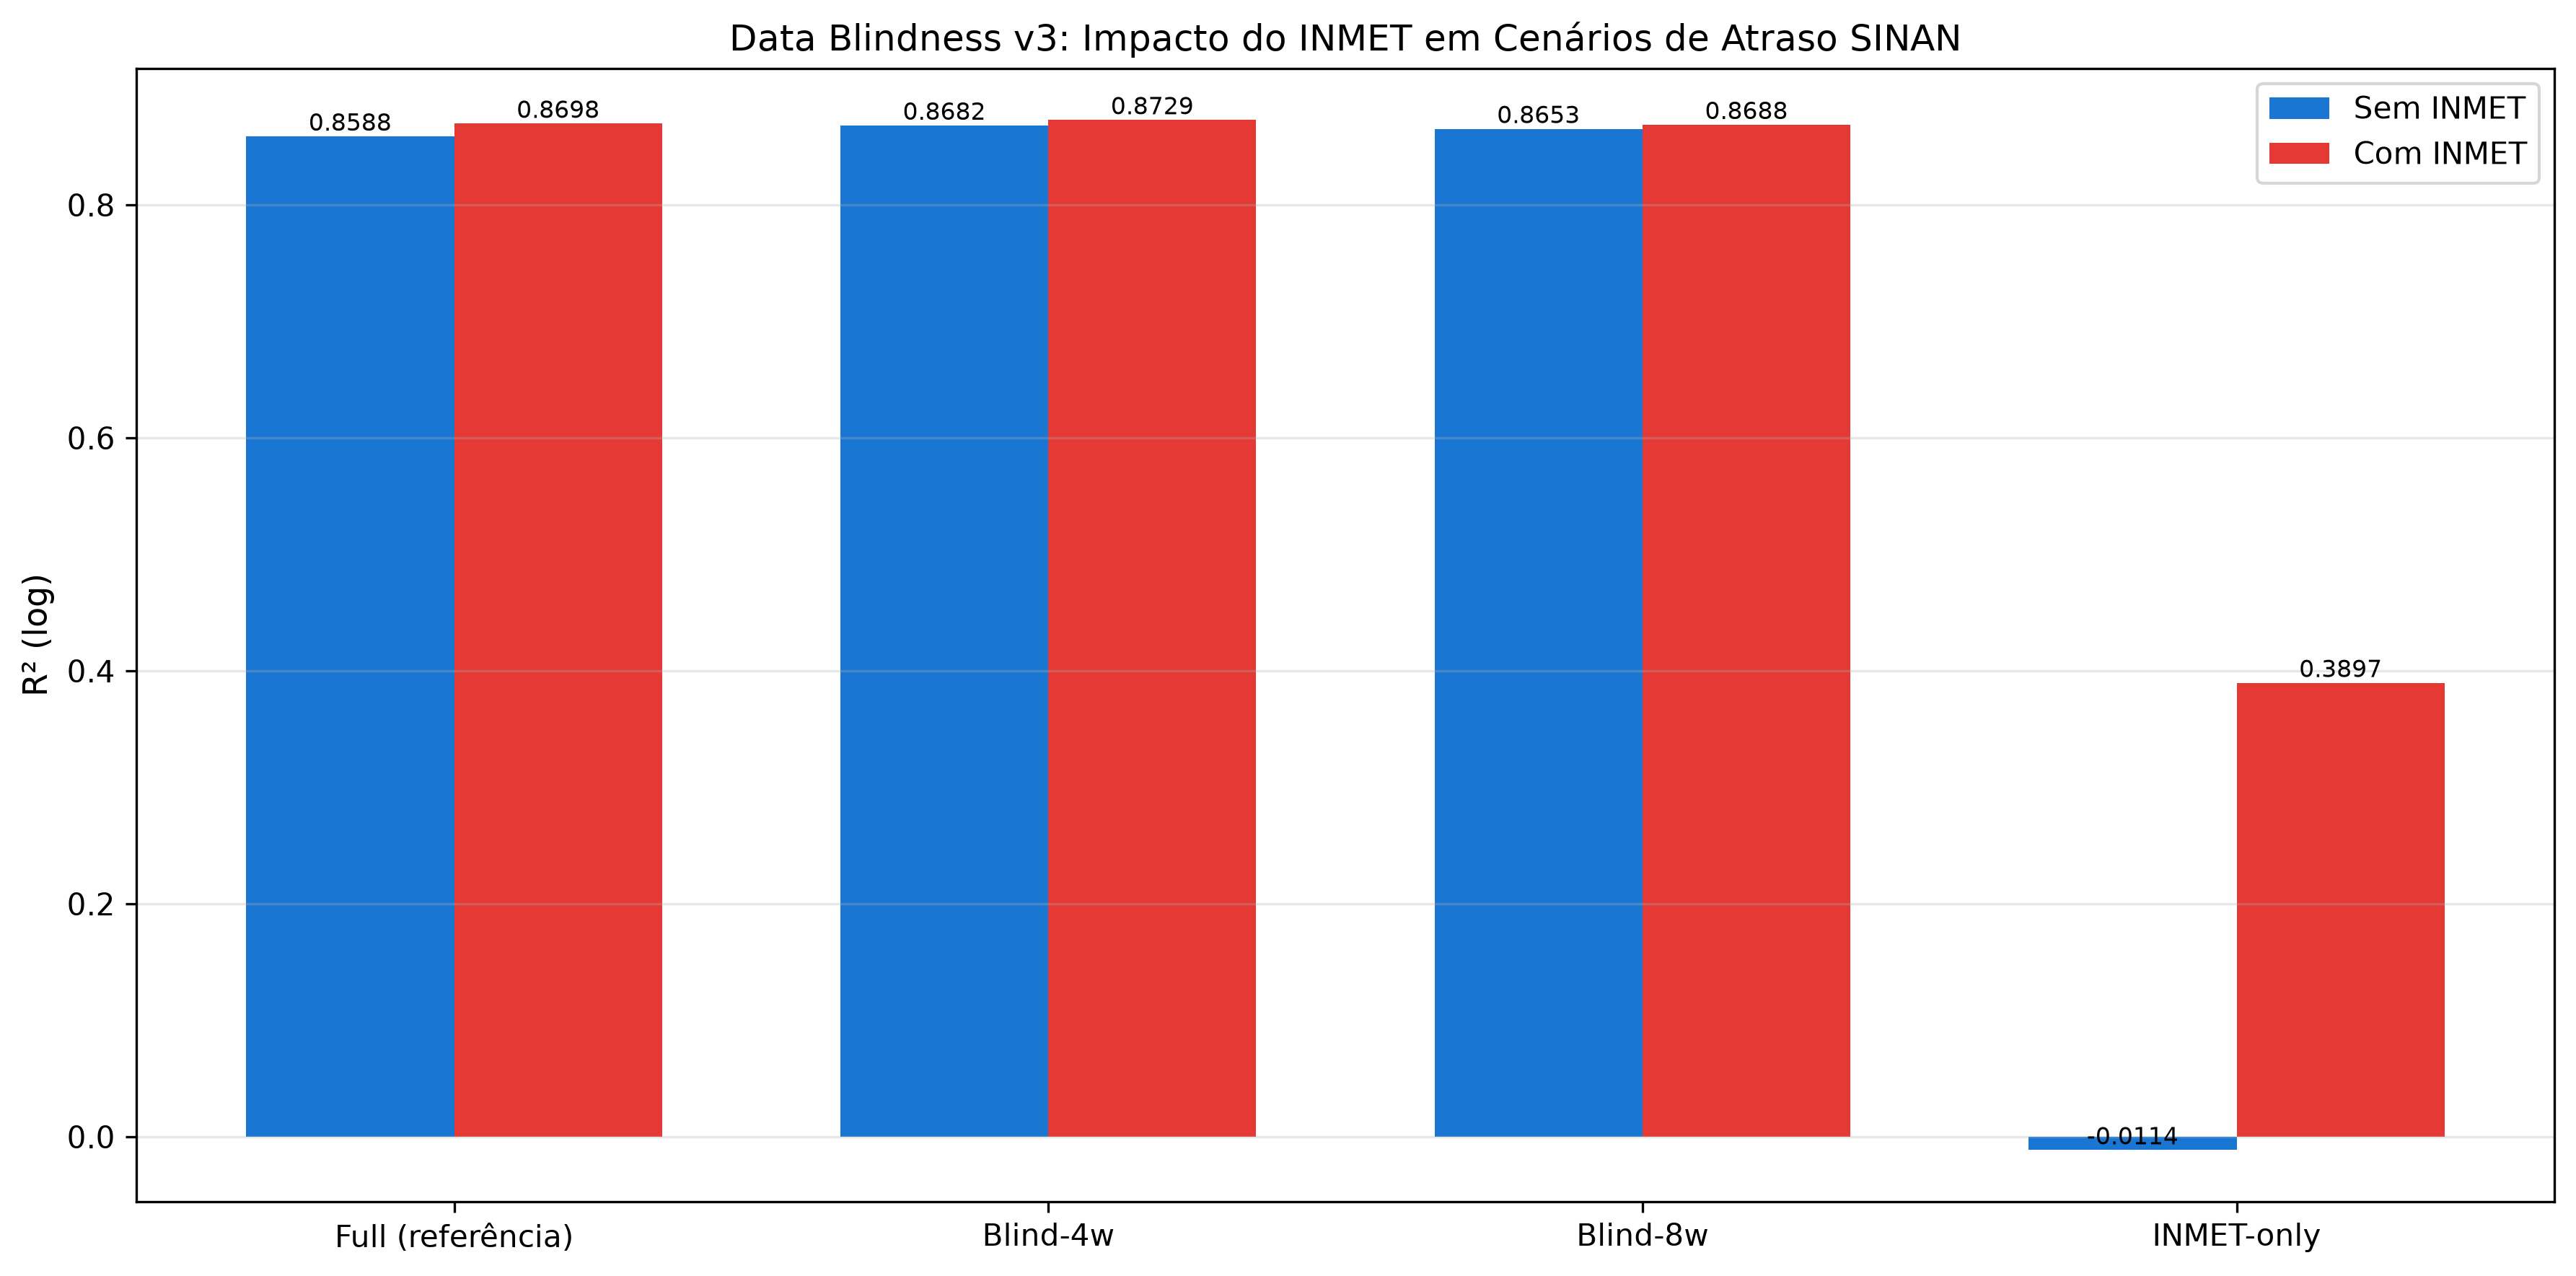
\includegraphics[width=0.9\textwidth]{figuras/resultados/fig_v3_blindness_comparison.png}
    \caption{$R^2_{\log}$ com e sem clima nos cenários de atraso na notificação --- pipeline v3}
    \label{fig:blindness_v3}
    \fonte{Dados do SINAN (DATASUS) e do INMET, 2000--2026.}
\end{figure}

Esses resultados devem ser lidos com a limitação apontada na metodologia: os cenários de atraso removem as defasagens de notificações, mas mantêm as contagens agregadas da semana $t$, como casos confirmados ou prováveis, o que explica por que o desempenho quase não cai. Uma simulação mais realista do atraso tenderia a reduzir o desempenho sem clima e a aumentar o valor relativo das variáveis climáticas.

\end{apendicesenv}
